\section{插入图片}
期刊论文很少有纯文字的叙述,很多情况下都要有图像加以证明。而\LaTeX 中插入图片也非常的方便,且接受tif 或 eps矢量图的格式。下面就介绍几种常见插入图片的格式。

\subsection{一般图片插入}
本节介绍单张图片的插入以及相关题注和交叉引用,在插入图片前需在导言区使用graphicx宏包。如图\ref{头像}
所示为单张图像的插入。需要注意的是需要插入的图片需要和tex 文件在同一个文件夹,为了方便管理也可指定文件夹,并把文章所需要的图片都放在相同文件夹内便于管理;需要插入的图片文件名不能存在中文字符。如果想实现图片包含题注以及可以交叉引用,则需要使用figure环境。

\begin{figure}[htbp]
	\centering
	\includegraphics[width=0.4\linewidth]{image}	% 图片的宽度为 0.4 倍的行宽
	\caption{头像}
	\label{头像}
\end{figure}

\subsection{含有子图的图片}
在期刊论文写作的过程中,可能单张图片无法满足想要达到的效果。更多情况下我们需要对多张图片进行综合分析或对比分析,因此本节主要分享三种包含子图的插入方式。
\subsubsection{多张图片一个题注}
本节介绍多张图片共用同一张标题,比如我用过很多张头像,而且我并不需要对头像进行分类说明,只需要概括说明,此实可以直接插入多张图片如图\ref{用过的头像},此时仅有一个题注。两个图片的位置距离都遵循段落格式的基本设置。

\begin{figure}[htbp]
	\centering
	\includegraphics[width=0.4\linewidth]{image} \hspace{1cm}	% 图片间隔 1cm
	
\includegraphics[width=0.4\linewidth]{gou}
	\caption{用过的头像}
	\label{用过的头像}
\end{figure}
\subsubsection{多张图片拥有小题注以及公共题注}
上节所表述的方法是针对于不需要区分子图情况,因此当需要区分子图的时候,例如引用某一个子图的时候,就需要在拥有公共题注的时候对每个子图进行命名,比如图\ref{情侣头像}
为情侣头像,图\ref{情侣狗}
为生肖为狗的头像,图\ref{生肖鼠}
为生效为鼠的头像。
\begin{figure}[htbp]
	\centering
	\subfigure[情侣狗]{\label{情侣狗}
\includegraphics[width=0.4\linewidth]{gou}} \quad
	\subfigure[情侣鼠]{\label{生肖鼠}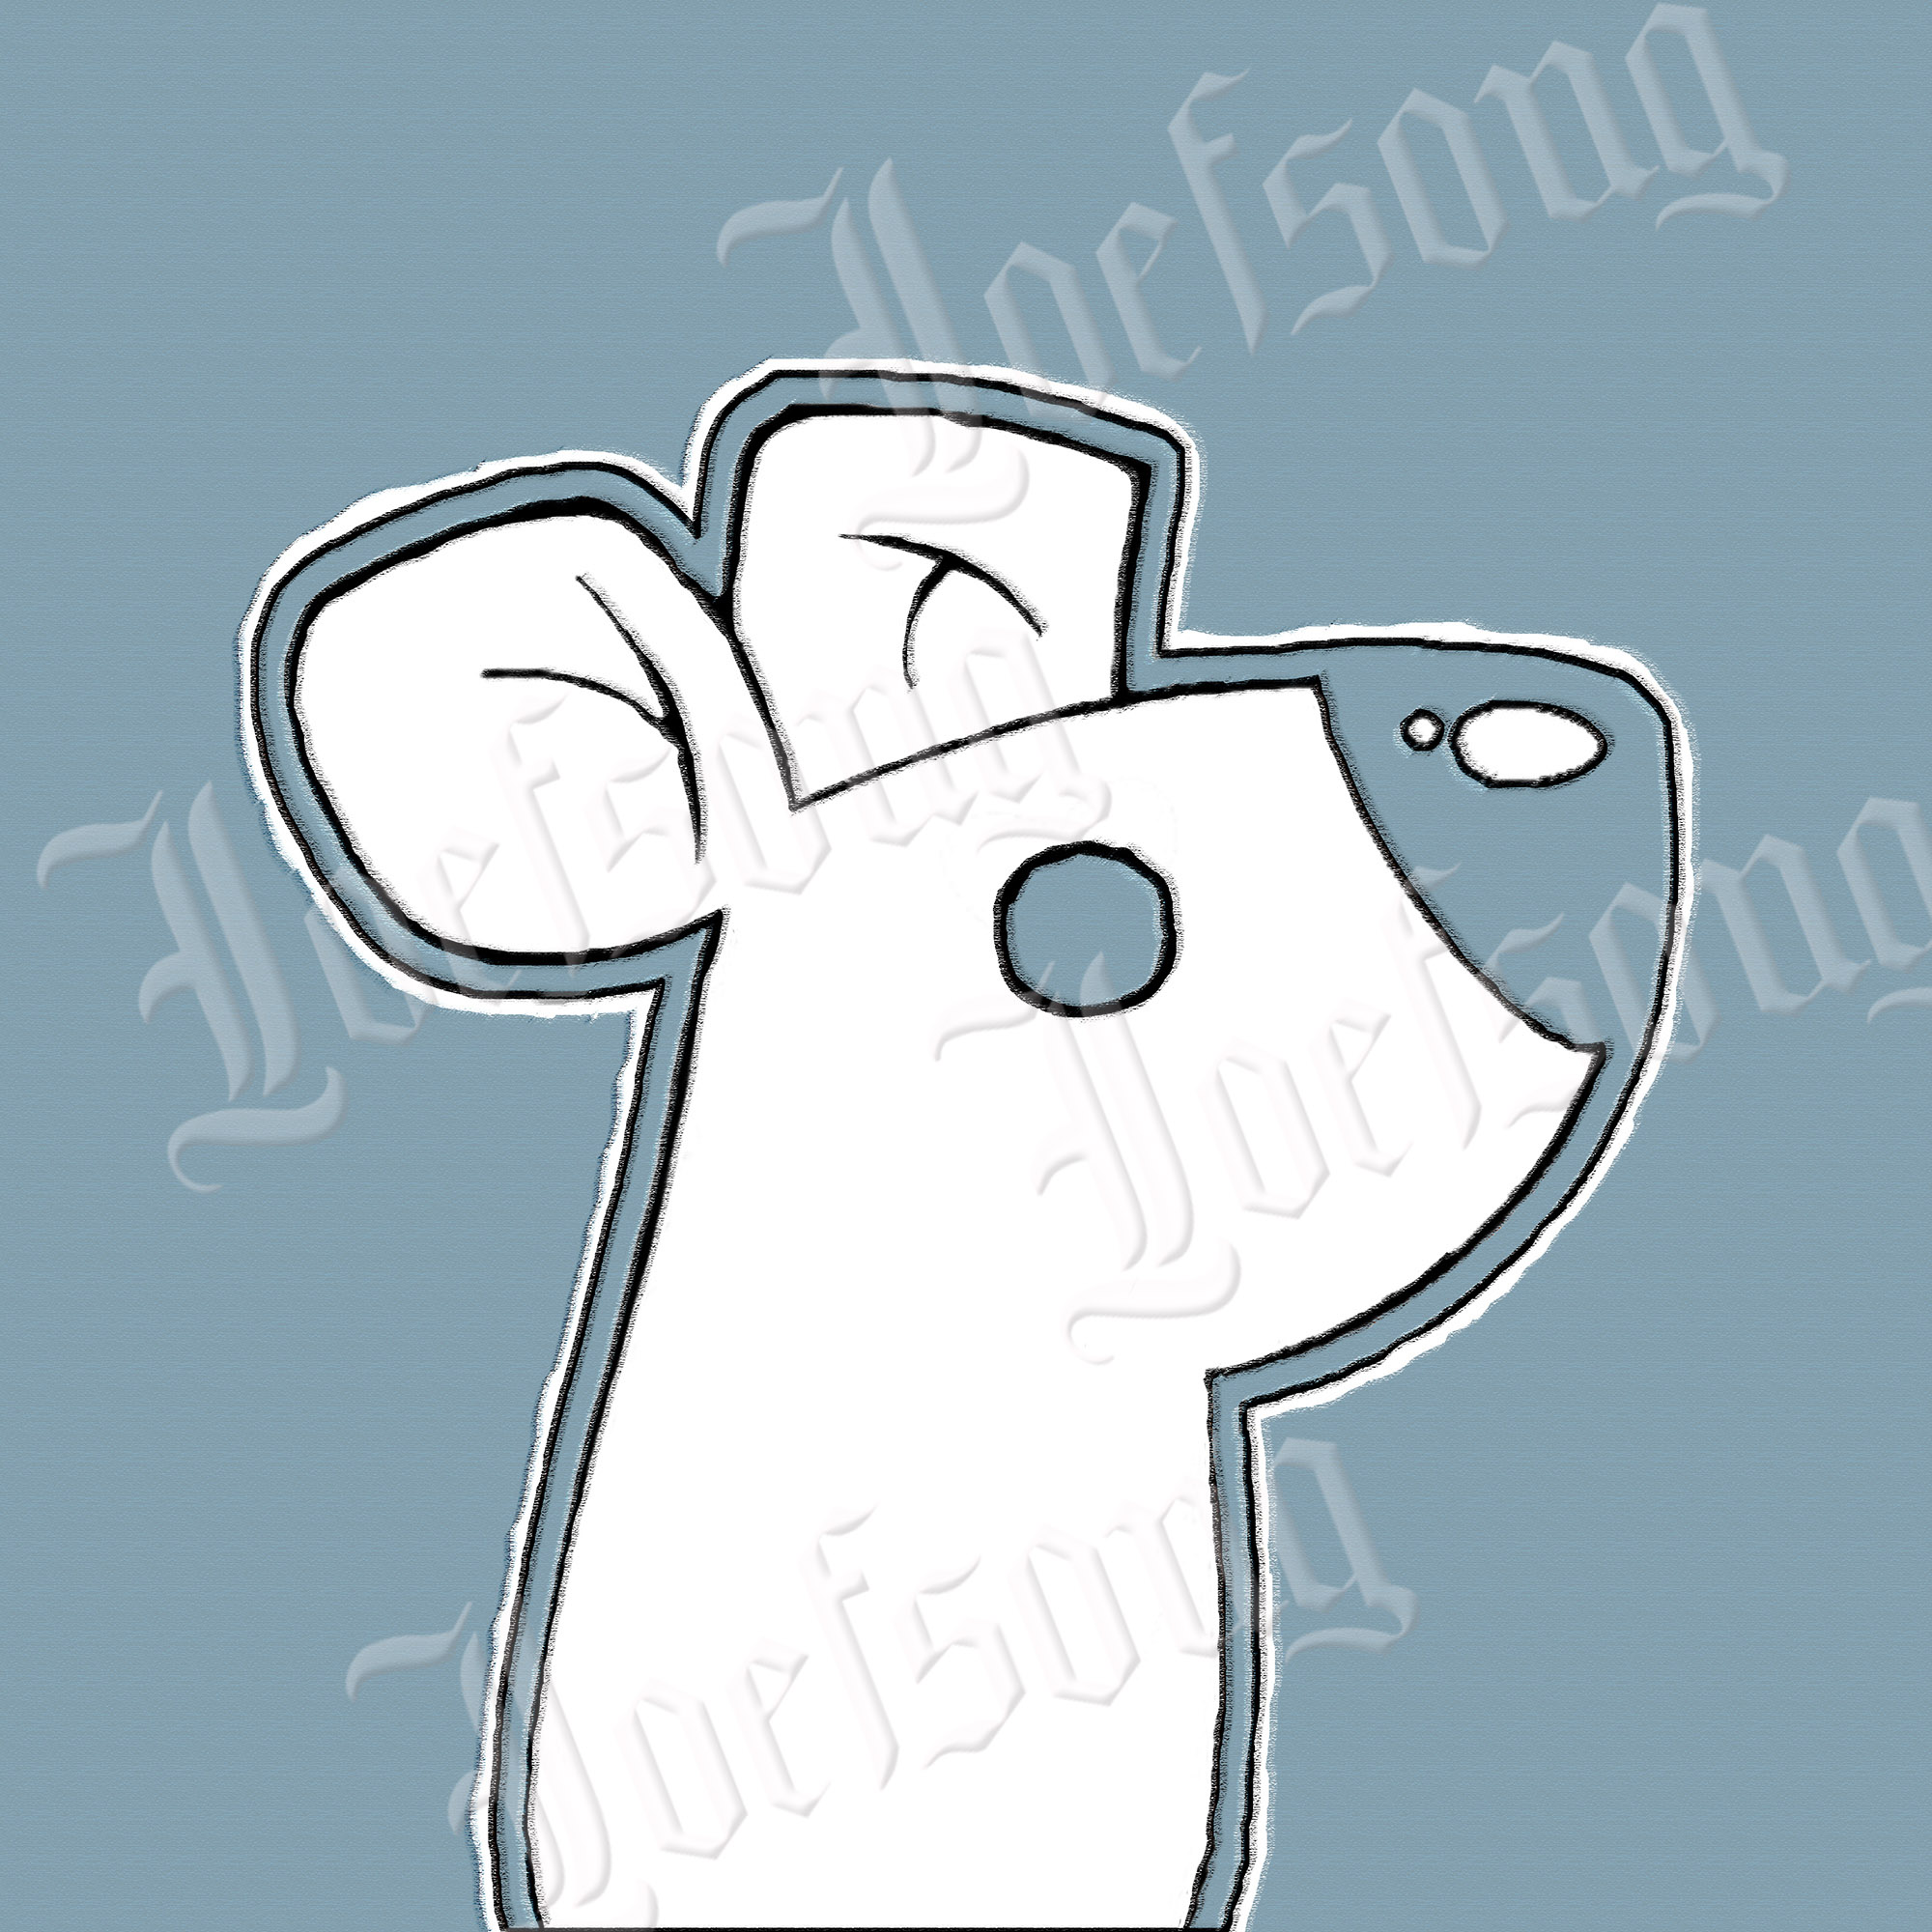
\includegraphics[width=0.4\linewidth]{shu}}
	\caption{情侣头像}
	\label{情侣头像}
\end{figure}
\subsubsection{多张图片并排显示拥有单独题注}
有时候并列图片并非是用来做综合分析或者差异分析的,也有可能只是为了减单个图片所占用的空间,因此需要是多个图片并排显示,并且分别有各自的题注。由于直接用figure环境,其题注都是居中显示且单独成段,因此需要借助minipage 的环境插入图片。 例如图\ref{生肖虎}
和图\ref{生肖鸡}
为并列显示的两张拥有各自题注的图片。
\begin{figure}[htbp]
	\centering
	\begin{minipage}[htbp]{0.48\linewidth}
		\centering
		
\includegraphics[width=0.8\linewidth]{hu}	% 0.8 是 minipage 的行宽
		\caption{生肖虎} \label{生肖虎}
	\end{minipage}
\begin{minipage}[htbp]{0.48\linewidth}
	\centering
	
\includegraphics[width=0.8\linewidth]{ji}
	\caption{生肖鸡} \label{生肖鸡}
\end{minipage}
\end{figure}